\documentclass[11pt,twoside,a4paper]{exam}
\usepackage[unboxed]{cwpuzzle}
\usepackage{graphicx}
\begin{document}
  
\begin{center}
\fbox{\fbox{\parbox{5.5in}{\centering
Beantworte die folgenden fragen richtig. Wenn der Platzt ausgeht nutzte dein Heft. Wenn Antworten ungewiss nutzte dein Handout.}}}
\end{center}
\vspace{0.1in}
\makebox[\textwidth]{Name und Klasse:\enspace\hrulefill}

\begin{questions}
\question Fuelle die Defintion aus. wenn du fehler machst schreib sie richtig ab.

\fillin ist eine chronische \fillin die sowohl Merkmale einer Allergie als auch einer \fillin aufweist.
Der Erkrankte reagier \fillin auf den Kleber \fillin mit einer chronisches \fillin der \fillin. Linderung verschaft
nur eine \fillin.
\end{questions}

\begin{questions}
\question
  Kreuze die richtigen Symptome an.
  \begin{checkboxes}
\choice Chronische Entzündung der Dünndarmschleimhaut
\choice Adipositas
\choice Entwicklungsstörungen
\choice Augenschmerzen
\choice Durchfall/Erbrechen
  \end{checkboxes}
\end{questions}

\begin{questions}
  \question Sortiere die schritte der Diagnose mithilfe von Zahlen.
  
  \begin{oneparcheckboxes}
    \choice{Dünndarmbiopsie}
    \choice{Verdacht}
    \choice{Bluttest}
  \end{oneparcheckboxes}
\end{questions}

\begin{questions}
  \question Der Erkrankte darf Gluten nicht essen. Gluten muss als Inhaltstoff in der Inhaltsanabe von Lebensmittel zu finden sein. Du siehst 3 Bilder A, B, und C kreuze an welchne fuer den Erkrankten geniessbar sind.
     \begin{oneparcheckboxes}
     ┊ \choice{A}
     ┊ \choice{B}
  ┊ \choice{C}
     \end{oneparcheckboxes}
\end{questions}

\begin{figure}[ht]
\center
  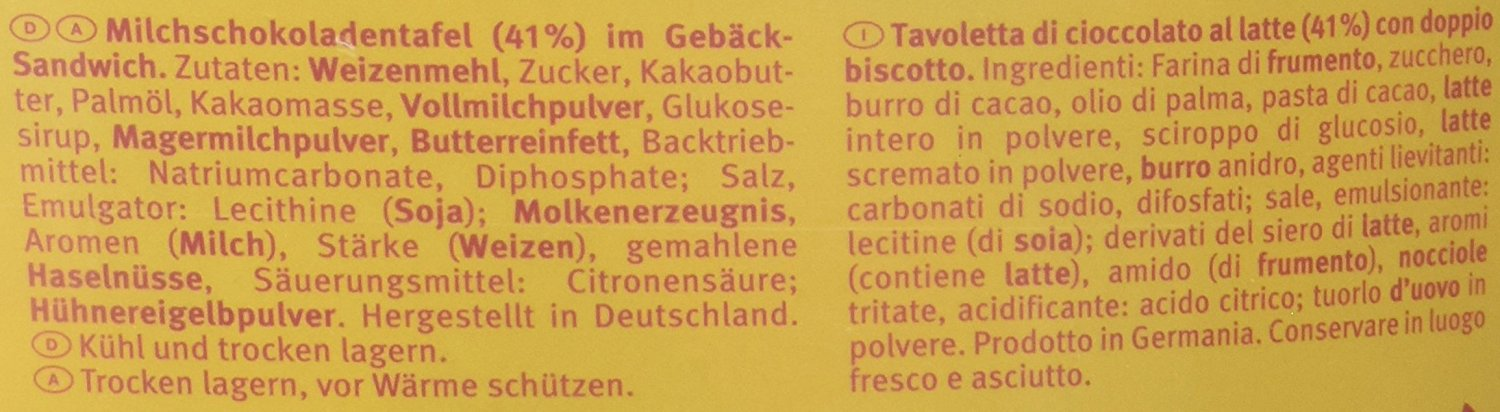
\includegraphics[width=0.7\textwidth, height=40px]{img/kekse.jpg}
	\caption{A}
\end{figure}

\begin{Puzzle}{16}{12}
|{}   |[1]O |[2]P |E  |R     |A  |T     |I  |O    |N  |{}    |{}   |[3]B |{} |{} |{} |.
|{}   |{}   |L    |{} |{}    |{} |{}    |{} |{}   |{} |{}    |[4]R |A    |N  |G  |E  |.
|[5]E |{}   |A    |{} |[6]M  |{} |{}    |{} |{}   |{} |{}    |{}   |R    |{} |{} |{} |.
|S    |{}   |[7]C |O  |O     |R  |D     |I  |N    |A  |T     |E    |G    |R  |I  |D  |.
|T    |{}   |E    |{} |D     |{} |{}    |{} |{}   |{} |{}    |{}   |R    |{} |{} |{} |.
|I    |{}   |V    |{} |E     |{} |{}    |{} |[8]V |A  |R     |I    |A    |B  |L  |E  |.
|[9]M |E    |A    |N  |{}    |{} |{}    |{} |{}   |{} |{}    |{}   |P    |{} |{} |{} |.
|A    |{}   |L    |{} |[10]L |I  |N     |E  |G    |R  |[11]A |P    |H    |{} |{} |{} |.
|T    |{}   |U    |{} |{}    |{} |{}    |{} |{}   |{} |X     |{}   |{}   |{} |{} |{} |.
|I    |{}   |E    |{} |{}    |{} |[12]S |C  |A    |L  |E     |M    |O    |D  |E  |L  |.
|O    |{}   |{}   |{} |{}    |{} |{}    |{} |{}   |{} |S     |{}   |{}   |{} |{} |{} |.
|N    |{}   |{}   |{} |{}    |{} |{}    |{} |{}   |{} |{}    |{}   |{}   |{} |{} |{} |.
\end{Puzzle}

\begin{PuzzleClues}{\textbf{Across}}
\Clue{1}{OPERATION}{Any mathematical process}
\Clue{4}{RANGE}{The lowest value in a set of numbers through the highest value in the set}
\Clue{7}{COORDINATEGRID}{A network of lines used for locating points}
\Clue{8}{VARIABLE}{Any symbol that could represent a number}
\Clue{9}{MEAN}{Average}
\Clue{10}{LINEGRAPH}{Graph that displays data using line segments}
\Clue{12}{SCALEMODEL}{A model or drawing based on a ratio}
\end{PuzzleClues}

\begin{PuzzleClues}{\textbf{Down}}
\Clue{2}{PLACEVALUE}{the positions of a single digit in the whole number}
\Clue{3}{BARGRAPH}{A graph that uses bars to display data}
\Clue{5}{ESTIMATION}{The use of rounding to determine a reasonable answer}
\Clue{6}{MODE}{The number found most often}
\Clue{11}{AXES}{The horizontal and vertical number lines used in a graph}
\end{PuzzleClues}

\end{document}
